% ------------------------------------------------------------------------------
% TYPO3 Version 9.3 - What's New - Chapter "Changes for Integrators" (English Version)
%
% @author	Michael Schams <schams.net>
% @license	Creative Commons BY-NC-SA 3.0
% @link		http://typo3.org/download/release-notes/whats-new/
% @language	English
% ------------------------------------------------------------------------------
% LTXE-CHAPTER-UID:		3a9852ea-e2360d9d-1ff5eec1-a7de3f9f
% LTXE-CHAPTER-NAME:	Changes for Integrators
% ------------------------------------------------------------------------------

\section{Modifiche per integratori}
\begin{frame}[fragile]
	\frametitle{Modifiche per integratori}

	\begin{center}\huge{Capitolo 2:}\end{center}
	\begin{center}\huge{\color{typo3darkgrey}\textbf{Modifiche per integratori}}\end{center}

\end{frame}

% ------------------------------------------------------------------------------
% LTXE-SLIDE-START
% LTXE-SLIDE-UID:		0e4cbd97-acee71f5-ac0a9fa4-94f3c684
% LTXE-SLIDE-TITLE:		...
% LTXE-SLIDE-REFERENCE:	#84843 - Use no-cookie domain for youtube by default
% ------------------------------------------------------------------------------

\begin{frame}[fragile]
	\frametitle{Modifiche per integratori}
	\framesubtitle{Dominio No-cookie per i video YouTube}

	% decrease font size for code listing
	\lstset{basicstyle=\smaller\ttfamily}

	\begin{itemize}
		\item I video YouTube sono di default renderizzati accedendo al dominio no-cookie
			\url{https://www.youtube-nocookie.com}
		\item Il dominio regolare \texttt{www.youtube.com} può essere forzato usando
			la seguente configurazione TypoScript, se richiesto:

			\begin{lstlisting}
				lib.contentElement {
				  settings {
				    media {
				      additionalConfig {
				        no-cookie = 0
				      }
				    }
				  }
				}
			\end{lstlisting}

	\end{itemize}

\end{frame}

% ------------------------------------------------------------------------------
% LTXE-SLIDE-START
% LTXE-SLIDE-UID:		64aaa747-fcd7919b-92dfd47f-65a3237c
% LTXE-SLIDE-TITLE:		General Data Protection Regulation
% LTXE-SLIDE-REFERENCE:	#84843 - Use no-cookie domain for youtube by default
% LTXE-SLIDE-REFERENCE:	GDPR Initiative: https://forge.typo3.org/issues/84776
% ------------------------------------------------------------------------------

\begin{frame}[fragile]
	\frametitle{Modifiche per integratori}
	\framesubtitle{General Data Protection Regulation - GDPR}

	\begin{itemize}
		\item Un task dello Scheduler può essere attivato per anonimizzare gli indirizzi IP 
			in vari punti delle tabelle del database dopo un certo periodo di tempo.\newline

			Per esempio le tabelle \texttt{sys\_log}, dopo 30 giorni:
			\begin{figure}
				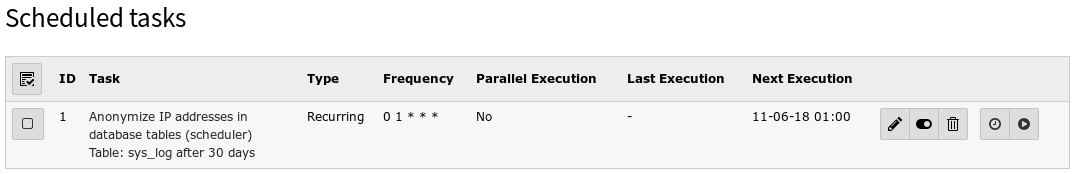
\includegraphics[width=1\linewidth]{ChangesForIntegrators/IpAnonymizationSchedulerTask.png}
			\end{figure}

		\item Il \href{https://typo3.com/blog/tag/gdpr/}{TYPO3 GmbH Blog}
			contiene maggiori informazioni riguardo il GDPR
	\end{itemize}

\end{frame}

% ------------------------------------------------------------------------------
% LTXE-SLIDE-START
% LTXE-SLIDE-UID:		b40d897b-8e020c70-d6f86717-54086093
% LTXE-SLIDE-TITLE:		FE/BE User Accounts and Passwords
% LTXE-SLIDE-REFERENCE:	#85026 - salted passwords changes
% ------------------------------------------------------------------------------

\begin{frame}[fragile]
	\frametitle{Modifiche per integratori}
	\framesubtitle{Utent FE/BE e password}

	% decrease font size for code listing
	\lstset{basicstyle=\tiny\ttfamily}

	\begin{itemize}
		\item Le password in chiaro non possono più essere usate per gli utenti BE/FE
		\item Gli utenti FE/BE inattivi possono essere rimossi dal database
			attivando il task scheduler "Table garbage collection task" e abilitando
			"Clean all available tables"\newline
			\smaller
				(i dati che non esistono non possono essere compromessi in caso di violazione
					della sicurezza)
			\normalsize

			\begin{lstlisting}
				<?php
				$tableGarbageCollectionTask = \TYPO3\CMS\Scheduler\Task\TableGarbageCollectionTask::class;
				$GLOBALS['TYPO3_CONF_VARS']['SC_OPTIONS']['scheduler']['tasks'][$tableGarbageCollectionTask]
				  ['options']['tables'] = [
				  'be_users' => [
				    'dateField' => 'lastlogin',
				    'expirePeriod' => 30
				  ]
				];
			\end{lstlisting}

		\item Vedi la \href{https://docs.typo3.org/typo3cms/extensions/scheduler/Installation/BaseTasks/Index.html}{documentazione}
			per maggiori dettagli
	\end{itemize}

\end{frame}

% ------------------------------------------------------------------------------
% LTXE-SLIDE-START
% LTXE-SLIDE-UID:		aee0dcee-251980b0-475e5557-4016bfde
% LTXE-SLIDE-TITLE:		"Duplicate" Button
% LTXE-SLIDE-REFERENCE:	#84749 - Hide "duplicate" button by default
% ------------------------------------------------------------------------------

\begin{frame}[fragile]
	\frametitle{Modifiche per integratori}
	\framesubtitle{Bottone "Duplica"}

	% decrease font size for code listing
	\lstset{basicstyle=\smaller\ttfamily}

	\begin{itemize}
		\item Il buttone per duplicare un elemento di contenuto è ora nascosto di default
		\item La sua visibilità può essere configurata in TSconfig ("1" = attiva):

			\begin{lstlisting}
				options.showDuplicate = 1
				options.showDuplicate.[table] = 1
			\end{lstlisting}

	\end{itemize}
	\vspace{-0.5cm}
	\begin{figure}
		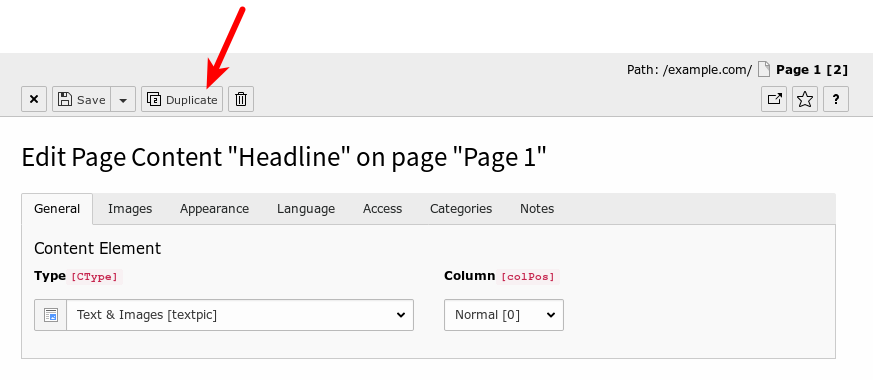
\includegraphics[width=0.8\linewidth]{ChangesForIntegrators/DuplicateButtonHiddenByDefault.png}
	\end{figure}

\end{frame}

% ------------------------------------------------------------------------------
% LTXE-SLIDE-START
% LTXE-SLIDE-UID:		78b3d97d-09272705-e529a6ee-bbdc1766
% LTXE-SLIDE-TITLE:		HTML5 Date Form Element
% LTXE-SLIDE-REFERENCE:	#82511 - EXT:form add HTML5 date form element
% ------------------------------------------------------------------------------

\begin{frame}[fragile]
	\frametitle{Modifiche per integratori}
	\framesubtitle{Elemento di form data in \texttt{EXT:form}}

	% decrease font size for code listing
	\lstset{basicstyle=\tiny\ttfamily}

	\begin{itemize}
		\item La struttura del Form dispone di un nuovo elemento di form "\texttt{Data}",
			inclusi validatori appropriati
		\item Questo è tecnicamente un elemento HTML5 con attributo \texttt{'type=date'}
			(vedi \href{https://www.w3.org/TR/2011/WD-html-markup-20110405/input.date.html}{w3c.org})
		\item Esempio (incluso il validatore "Intervallo di date"):

			\begin{lstlisting}
				type: Date
				identifier: date-1
				label: Date
				defaultValue: '2018-03-02'
				properties:
				  displayFormat: 'd.m.Y'
				  fluidAdditionalAttributes:
				    min: '2018-03-01'
				    max: '2018-03-30'
				    step: '1'
				validators:
				  -
				    identifier: DateRange
				    options:
				      minimum: '2018-03-01'
				      maximum: '2018-03-30'
			\end{lstlisting}

	\end{itemize}

\end{frame}

% ------------------------------------------------------------------------------
% LTXE-SLIDE-START
% LTXE-SLIDE-UID:		e60b0276-13632d81-701999f3-8e59ab2e
% LTXE-SLIDE-TITLE:		Destructive Database Schema Changes
% LTXE-SLIDE-REFERENCE:	#85160 - Non destructive database schema changes in extension manager
% ------------------------------------------------------------------------------

\begin{frame}[fragile]
	\frametitle{Modifiche per integratori}
	\framesubtitle{Modifica distruttive della struttura del database}

	\begin{itemize}
		\item Se un estensione è installata o aggiornata via l'Extension Manager,
			e sono necessari dei cambiamenti \textit{distruttivi}, questi cambiamenti
			non sono più applicati in automatico
		\item Cambiamenti "distruttivi" sono per esempio cambiamenti delle colonne esistenti,
			rimozione di un colonna, definizione degli indici di una tabella, ecc.
		\item Per rivedere ed eventualmente eseguire questi aggiornamenti del database in sospeso,
			accedere a: ADMIN TOOLS → Manutenzione → Analizza struttura database\newline
	\end{itemize}

	\vspace{-0.4cm}

	% Translators: remove the illustration below, if it does not fit on the
	% slide, e.g. in case your language requires more space. The illustration is
	% not really required, just "nice to have".

	\begin{figure}
		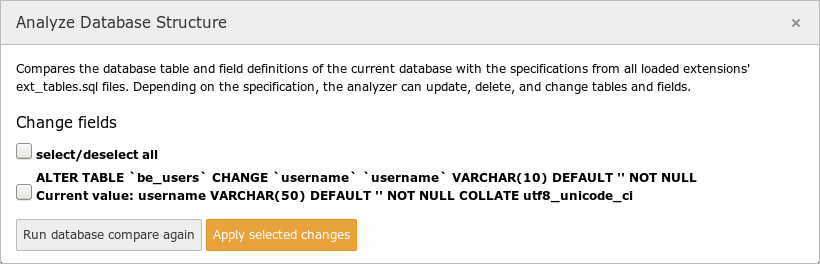
\includegraphics[width=0.6\linewidth]{ChangesForIntegrators/DestructiveDatabaseChanges.png}
	\end{figure}

\end{frame}

% ------------------------------------------------------------------------------
% LTXE-SLIDE-START
% LTXE-SLIDE-UID:		38dadab3-c11b6d58-126f6ed4-18ac5e69
% LTXE-SLIDE-TITLE:		TypoScript Conditions
% LTXE-SLIDE-REFERENCE:	#84760 - TypoScript conditions for site and siteLanguage
% ------------------------------------------------------------------------------

\begin{frame}[fragile]
	\frametitle{Modifiche per integratori}
	\framesubtitle{Condizioni TypoScript}

	Nuove condizioni TypoScript:

	\begin{itemize}
		\item Condizione per le proprietà di un oggetto sito

			\begin{lstlisting}
				[site = identifier = someIdentifier, base = https://example.com/]
				  page.30.value = foo
				[global]
			\end{lstlisting}

		\item Condizione per la lingua di un sito

			\begin{lstlisting}
				[siteLanguage = locale = de_CH.UTF-8, title = Switzerland]
				  page.40.value = bar
				[global]
			\end{lstlisting}

	\end{itemize}

\end{frame}

% ------------------------------------------------------------------------------
% LTXE-SLIDE-START
% LTXE-SLIDE-UID:		e72af588-a2aaef44-bb8a1703-f25ca002
% LTXE-SLIDE-TITLE:		HMENU cObj and language IDs
% LTXE-SLIDE-REFERENCE:	#84775 - Extend HMENU to support auto filling of special.value for special=language
% ------------------------------------------------------------------------------

\begin{frame}[fragile]
	\frametitle{Modifiche per integratori}
	\framesubtitle{cObj \texttt{HMENU} e ID di lingua}

	% decrease font size for code listing
	%\lstset{basicstyle=\tiny\ttfamily}

	\begin{itemize}
		\item l'oggeto di contenuto \texttt{HMENU} ora supporta l'autocompletamento 
			dell'ID di linguaggio per il menu di lingua

			\begin{lstlisting}
				10 = HMENU
				10 {
				  special = language
				  special.value = auto
				}
  			\end{lstlisting}

		\item \texttt{special.value} vuole una lista separata da virgole di ID
			(es. 0,1,2) o \texttt{auto} per caricare la lista dalle lingue del sito

	\end{itemize}

\end{frame}

% ------------------------------------------------------------------------------
% LTXE-SLIDE-START
% LTXE-SLIDE-UID:		9cdf141c-8e244da5-e79cca00-4964a18b
% LTXE-SLIDE-TITLE:		View User TSConfig Data
% LTXE-SLIDE-REFERENCE:	#85017 - User TSConfig shown in Configuration module
% ------------------------------------------------------------------------------

\begin{frame}[fragile]
	\frametitle{Modifiche per integratori}
	\framesubtitle{Visualizza i dati del TSconfig Utente}

	I dati del TSConfig Utente dell'utente attualmente collegato possono essere visti in
	\textbf{Sistema -> Configurazione}

	\begin{figure}
		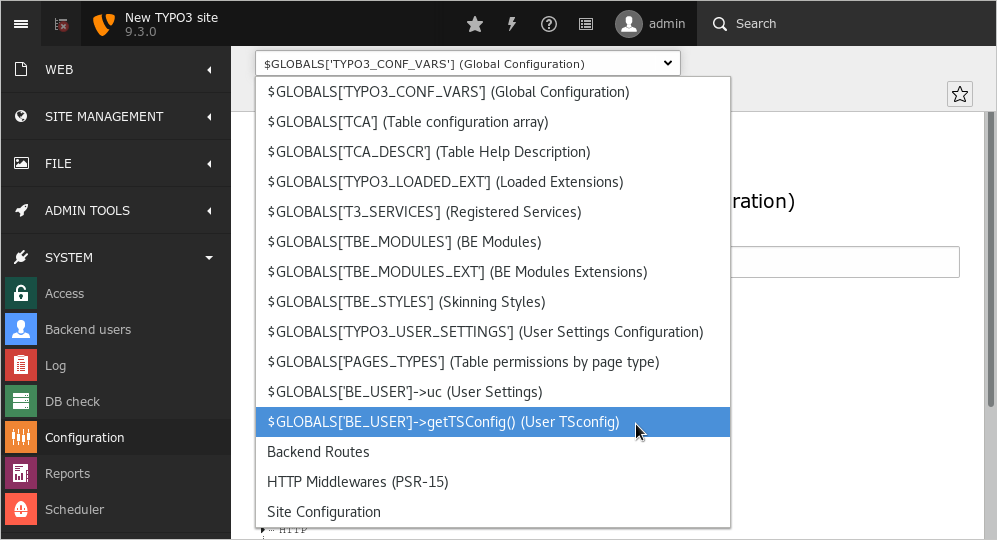
\includegraphics[width=0.75\linewidth]{ChangesForIntegrators/SystemConfigurationUserTSConfig.png}
	\end{figure}

\end{frame}

% ------------------------------------------------------------------------------
% LTXE-SLIDE-START
% LTXE-SLIDE-UID:		a2b0fb75-abe28977-37e4115d-1d73f99e
% LTXE-SLIDE-TITLE:		Miscellaneous
% LTXE-SLIDE-REFERENCE:	#69274 - Preserve image rotation if orient is saved in exif
% LTXE-SLIDE-REFERENCE:	#85147 - Render SEO meta tags in frontend
% LTXE-SLIDE-REFERENCE:	#84715 - Set exclude property for tt_content fields
% ------------------------------------------------------------------------------

\begin{frame}[fragile]
	\frametitle{Modifiche per integratori}
	\framesubtitle{Varie}

	\begin{itemize}
		\item TYPO3 considera l'orientamento dell'immagine memorizzato nei dati EXIF,
			durante la lettura delle dimensioni e l'elaborazione dell'immagine (es. ridimensionamento/crop)
		\item I meta tag relativi al SEO impostati nelle proprietà di pagina sono ora renderizzati
			in frontend di default
		\item La proprietà \textit{exclude} è impostata per i seguenti campi:

			\begin{itemize}
				\smaller
				\item \texttt{tt\_content.file\_collections}
				\item \texttt{tt\_content.filelink\_size}
				\item \texttt{tt\_content.filelink\_sorting}
				\item \texttt{tt\_content.filelink\_sorting\_direction}
			\end{itemize}

			\small
				I permessi di Accesso devono essere aggiustati, se l'editore deve essere in grado 
				di vedere questi campi!
			\normalsize

	\end{itemize}

\end{frame}

% ------------------------------------------------------------------------------
